\documentclass[a4paper]{article}
\usepackage{exercise}
%um nur aufgaben zu zeigen
%\usepackage[noanswer]{exercise} 
\usepackage{../images/preamble}


\begin{document}
	\vspace*{-2cm}
	\parbox{4cm}{
\includegraphics[width=2.5cm]{../images/ROLF4.png}}
	\parbox{10.6cm}{\setstretch{2.0} \centering{ \huge \textsf{Widerstände und Bewegungen}}\\18. Januar 2017 \\ \href{mailto:physikrolf@gmail.com}{physikrolf@gmail.com},~\url{pankratius.github.io/rolf}\\ \vspace*{-.5cm} }
	
	

\thispagestyle{empty}

\noindent
\begin{Exercise}[label = wdsw, title = Widerstandswürfel , difficulty = 2, origin ={}]
	Gegeben ist ein Würfel, wobei jede der Kanten einen Widerstand von $R = 1~\mathrm{\Omega}$ hat.\\
	Wie groß ist der Widerstand entlang einer Raumdiagonale?
\end{Exercise}
\begin{Answer}[ref=wdsw]
	Wir wollen den Widerstand zwischen den Punkten $X$ und $Y$ bestimmen, also entlang der Raumdiagonale (siehe Abb. \ref{fig:wdsws1}). Weil die Raumdiagonale eine Symmetrieachse ist, sollte das Problem symmetrisch sein, und deswegen eine recht einfache Lösung haben.\\
	Um die zu finden, schauen wir uns die Punkte $a$ und $b$ an, die jeweils den gleichen Abstand von $X$ und $Y$ haben. Diese müssen jeweils auf dem gleichen Potential liegen. Um zu sehen, warum das so ist, stellen wir uns vor, dass der Strom $I$ aus dem Punkt $X$ in die drei Punkte $a$ fließt. Weil alle drei Punkte gleich weit von $X$ entfernt sind (bzw. zwischen jedem Punkt $a$ und $X$ jeweils der Widerstand $R$ ist), muss sich der Strom gleichmäßig aufteilen. Gleichzeitig ist aber jeder Punkt $a$ mit zwei Punkten $b$ verbunden ist, muss sich auch hier der Strom gleichmäßig aufteilen. Also müssen alle Punkte $a$ auf dem gleichen Potential liegen, und auch alle Punkte $b$ auf einem anderen selben Potential.\\
	Damit können wir einen neuen Stromkreis zeichnen, in dem es nur einen Punkt $a$ und nur einen Punkt $b$ gibt, siehe Abb. \ref{fig:wdsws2}. Dieser ist eine einfache Schaltung von Widerständen, die alle den Wert $R$ haben. Werten wir die einzelnen Parallelschaltungen aus, so trägt die ersten einen Wert von $\frac{R}{3}$ bei, und die zweite einen Wert von $\frac{R}{6}$ und die dritte wieder $\frac{R}{3}$. Der Gesamtwiderstand ergibt sich aus der Reihenschaltung der drei, also $R_g = 2\cdot \frac{R}{3}+ \frac{R}{6} = \frac{5R}{6}$.
	

\end{Answer}
\begin{figure}[h]
\begin{subfigure}[b]{0.4\textwidth}
	\centering
	
	\tdplotsetmaincoords{80}{120}
\begin{tikzpicture}[scale=3, tdplot_main_coords,axis/.style={->},thick]  

    \coordinate (O) at (0,0,0);
    \tdplotsetcoord{P}{1.414213}{54.68636}{45}
    
    \draw (O) -- (Py) -- (Pyz) -- (Pz) -- cycle;
    \draw(O) -- (Px) -- (Pxy) -- (Py) -- cycle;
    \draw (O) -- (Px) -- (Pxz) -- (Pz) -- cycle;
    \draw(Pz) -- (Pyz) -- (P) -- (Pxz) -- cycle;
    \draw (Px) -- (Pxy) -- (P) -- (Pxz) -- cycle;
    \draw (Py) -- (Pxy) -- (P) -- (Pyz) -- cycle;
    \node at (0,-0.1,0.05) {$Y$};
    \node at (1,1,0.8) {$X$};
    \node at (-0.15,-0.1,0.875){$b$};
    \node at (1,0,0.85){$a$};
    \node at (-0.1,0.8,0.87){$a$};
    \node at (1,1,-0.01){$a$};
    \node at (0,0.9,0){$b$};
    \node at (1,0.05,-0.01){$b$};
	\foreach \x in {0,0.82}
	\foreach \y in {0,0.82}
	\foreach \z in {0,0.82}
	 {\draw[fill=black] (\x,\y,\z) circle (0.5pt);}    

\end{tikzpicture}

	\caption{Skizze des Wurfels}
	\label{fig:wdsws1}
\end{subfigure}
\begin{subfigure}[b]{0.6\textwidth}
	\centering
	\begin{circuitikz} \draw
	(0,0) to (0.5,0)
	(0.5,-0.5) to (0.5,0.5)
	\foreach \h in {-0.5,0,0.5}
		{(0.5,\h) to[R] (2.5,\h)}
	(2.5,0.5) to (2.5,-0.5)
	(2.5,0) to (3,0)	
 	(3,-1.5) to (3,1.5)
	\foreach \h in {-1.5,-1,-0.5,0.5,1,1.5}
	{(3,\h) to[R] (5,\h)}
	(5,1.5) to (5,-1.5)
	(5,0) to (6,0)
	(6,-0.5) to (6,0.5)
	\foreach \h in {-0.5,0,0.5}
	{(6,\h) to[R] (8,\h)}
	(8,0.5) to (8,-.5)
	(8,0) to (8.5,0)
	;
	\node at (-0.2,0) {$X$};
	\filldraw[black] (0,0) circle (1.5pt);
	\node at (8.7,0) {$Y$};
	\filldraw[black] (8.5,0) circle (1.5pt); 
	\node at (2.75,0.3) {$a$};
	\filldraw[black] (2.75,0) circle (1.5pt);
	\node at (5.5,0.3) {$b$};
	\filldraw[black] (5.5,0) circle (1.5pt);
\end{circuitikz}
	\caption{vereinfachtes Schaltbild}
	\label{fig:wdsws2}
\end{subfigure}
\caption{Schaltskizzen zum Aufbau}
\end{figure}

\flushleft
\begin{minipage}{.57\textwidth}
\begin{Exercise}[label = wdsstrecke, title = Widerstandsstrecke, difficulty = 3, origin = IPhO 1996 ]
Bestimme den Widerstand zwischen den Punkten $A$ und $B$
	\end{Exercise}
\end{minipage}
\hfill
\begin{minipage}{.2\textwidth}
	\flushleft
	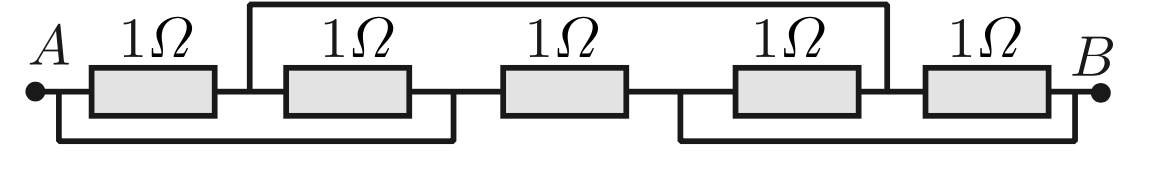
\includegraphics[scale = .2]{../tasks/ipho/wdsstrecke.png}
\end{minipage}
\begin{Answer}[ref = wdsstrecke]
	Um die Aufgabe einfach lösen zu können, muss man wissen, dass wen zwei Punkte nur durch einen Draht verbunden sind, sie auf dem gleichen Potential liegen müssen. Das liegt einfach daran, dass über ihnen keine Spannung abfallen kann, weil nichts da ist, an dem Spannung abfallen könnte \footnote{Außer natürlich der Draht selber. Aber in fast allen Aufgaben geht man davon aus, dass Drähte widerstandsfrei sind. Wenn das nicht so ist, sollte es auch angegeben sein.}\\
	Wir nennen diese Punkte $A$, $B$ und $C$ (siehe Abb.\ref{fig:wdsstreckeep}). Jetzt kann man einfach einen Stromkreis zeichnen, in dem es nur noch die Punkte $A$, $B$ und $C$ gibt. Dafür ist es hilfreich, wenn man die Widerstände nummeriert, sodass man sich nicht vertut. Wenn wir uns \ref{fig:wdsstreckeep} anschauen, dann stellen wir zuerst fest, dass $A$ mit $C$ durch die Widerstände 1 und 2 verbunden ist, $A$ mit $B$ durch 3 und $B$ mit $C$ durch die Widerstände $4$ und $5$. \\
	Der neue Stromkreis sieht dann so aus, wie in Abb.\ref{fig:wdsstreckes} gezeigt. Hier können wir jetzt mit den ganz normalen Regeln für Reihen- und Parallelschaltungen arbeiten. Die Widerstände 4 und 5 sind parallel geschaltet, die Widerstände 1 und 2 auch, und die Ersatzwiderstände für diese beiden Parallelschaltungen sind gemeinsam in Reihe parallel zu dem Widerstand 3 geschaltet.
	Damit ist der Gesamtwiderstand
	\begin{equation*}
		\boxed{
			\frac{1}{R_{AB}} =\underbrace{\frac{1}{R}}_{Wds. 3} + \overbrace{\frac{1}{\underbrace{\frac{R}{2}}_{1\parallel 2}+\underbrace{\frac{R}{2}}_{4\parallel 5}}}^{Wds.~parallel~zu~3} \Rightarrow R_{AB} = \frac{R}{2} = 0.5~\Omega,
			}
	\end{equation*}
	wobei mit einem Einzelwiderstand von $ R = 1~\Omega$ gerechnet wurde, wie in der Skizze zur Aufgabenstellung gezeigt.
\end{Answer}
\begin{figure}[h]
	\begin{subfigure}[b]{0.5\textwidth}
		\centering
		  \ctikzset{bipoles/resistor/width=0.4}
\begin{tikzpicture}
	\draw
		\foreach \h in {1,2,3,4,5}
		{(\h-1,0) to[/tikz/circuitikz/bipoles/length=25pt, R] (\h,0)};
	\foreach \h in {0,1,2,3,4,5}
	{\filldraw[black] (\h,0) circle (1.5pt);}
	\node at (-0.2,0) {$A$};
	\node at (5.2,0) {$B$};
	\node at (1,0.3){$C$};
	\node at (2,-0.3){$A$};

	\node at (3,-0.3) {$B$};
	\node at (4,0.3) {$C$};
	\draw (0,0) -- (0,0.5) -- (2,.5)--(2,0);
	\draw (1,0) -- (1,-.5) -- (4,-.5) -- (4,0);
	\draw (3,0) -- (3,.5) -- (5,.5)--(5,0);
	\foreach \h in {1,2,3,4,5}
	{\node at (-0.5+ \h,0) {\footnotesize \h};}

	
	 
	

\end{tikzpicture}
		\caption{Punkte auf gleichem Potential}
		\label{fig:wdsstreckeep}
	\end{subfigure}
	\begin{subfigure}[b]{0.5\textwidth}
		\centering
		  \ctikzset{bipoles/resistor/width=0.4}
\begin{tikzpicture}
	\draw
	(0,0) to[/tikz/circuitikz/bipoles/length=25pt, R] (1,0)
	(0,-0.5) to[/tikz/circuitikz/bipoles/length=25pt, R] (1,-0.5)
	(1,0) to (1.5,0)
	(0,0) to (0,-0.5)
	(1,-.5) to (1,0)
	(0,-.5) to (0,-1)
	(0,-1) to[/tikz/circuitikz/bipoles/length=25pt, R] (1.5,-1)
	(1.5,-1)to[/tikz/circuitikz/bipoles/length=25pt, R](1.5,0)
	(1.5,0) to (2,0)
	(1.5,-1) to (2,-1)
	(2,0) to[/tikz/circuitikz/bipoles/length=25pt, R] (2,-1)
	;
	\filldraw[black] (0,0) circle (1.5pt);
	\filldraw[black] (1,0) circle (1.5pt);
	\filldraw[black] (1.5,-1) circle (1.5pt);
	\node at (0,0.3) {$A$};
	\node at (1,0.3) {$C$};
	\node at (1.5,-1.3) {$B$};
	\node at (0.5,0) {\footnotesize 1};
	\node at (0.5,-.5) {\footnotesize 2};
	\node at (0.75,-1) {\footnotesize 3};
	\node at (1.5,-0.5) {\footnotesize 4};
	\node at (2,-0.5){\footnotesize 5};
	
\end{tikzpicture}
		\caption{vereinfachter Stromkreis}
		\label{fig:wdsstreckes}	
	\end{subfigure}
	\caption{Skizzen zum Aufbau}
\end{figure}
	

\flushleft
\begin{minipage}{.7\textwidth}
\begin{Exercise}[label = wdsss, title = Widerstandssechsecks, difficulty = 3, origin = Jaan Kalda ]
		Die nebenstehende Abbildung zeigt ein regelmäßiges Sechseck. Jede Seite des Sechseck hat den Widerstand $R= 1~\Omega$. Zudem ist jeder Eckpunkt des Sechsecks mit dem Mittelpunkt des $O$ verbunden, wobei jedes Verbindungsstück ebenfalls den Widerstand $R = 1 ~\Omega$.\\
		Berechne den Widerstand zwischen den Punkten $A$ und $O$.
	\end{Exercise}
\end{minipage}
	\definecolor{ttqqqq}{rgb}{0.2,0.,0.}
	\definecolor{sqsqsq}{rgb}{0.12549019607843137,0.12549019607843137,0.12549019607843137}
	\definecolor{uuuuuu}{rgb}{0.26666666666666666,0.26666666666666666,0.26666666666666666}
	\hfill
	\begin{minipage}{.25\textwidth}
		\centering
	\begin{tikzpicture}[line cap=round,line join=round,>=triangle 45,x=1.0cm,y=1.0cm]
	\clip(-0.978433710067438,-0.362269667894218) rectangle (2.184310516415405,2.2170027788754108);
 (0.,0.) -- (1.,0.) -- (1.5,0.8660254037844387) -- (1.,1.7320508075688776) -- (0.,1.7320508075688779) -- (-0.5,0.8660254037844395) -- cycle;
	\draw [color=ttqqqq] (0.,0.)-- (1.,0.);
	\draw [color=ttqqqq] (1.,0.)-- (1.5,0.8660254037844387);
	\draw [color=ttqqqq] (1.5,0.8660254037844387)-- (1.,1.7320508075688776);
	\draw [color=ttqqqq] (1.,1.7320508075688776)-- (0.,1.7320508075688779);
	\draw [color=ttqqqq] (0.,1.7320508075688779)-- (-0.5,0.8660254037844395);
	\draw [color=ttqqqq] (-0.5,0.8660254037844395)-- (0.,0.);
	\draw (0.,0.)-- (1.,1.7320508075688776);
	\draw (0.,1.7320508075688779)-- (1.,0.);
	\draw (-0.5,0.8660254037844395)-- (1.5,0.8660254037844387);
	\begin{scriptsize}
	\draw [fill=uuuuuu] (0.,0.) circle (1.5pt);
	\draw[color=uuuuuu] (-0.05142247127074252,-0.19636223384815558) node {$A$};
	\draw [fill=sqsqsq] (1.,0.) circle (1.5pt);
	\draw[color=sqsqsq] (1.1046150735816072,-0.1418321609777617) node {$B$};
	\draw [fill=uuuuuu] (1.5,0.8660254037844387) circle (1.5pt);
	\draw[color=uuuuuu] (1.6790267075540336,0.9355460664211556) node {$C$};
	\draw [fill=uuuuuu] (1.,1.7320508075688776) circle (1.5pt);
	\draw[color=uuuuuu] (1.1664440225723315,1.8534802396344964) node {$D$};
	\draw [fill=uuuuuu] (0.,1.7320508075688779) circle (1.5pt);
	\draw[color=uuuuuu] (0.030372638034848243,1.9298392614956145) node {$E$};
	\draw [fill=uuuuuu] (-0.5,0.8660254037844395) circle (1.5pt);
	\draw[color=uuuuuu] (-0.625834105243169,0.9573580955693131) node {$F$};
	\draw [fill=uuuuuu] (0.5,0.866025403784439) circle (1.5pt);
	\draw[color=uuuuuu] (0.7192974250351018,0.979990737081949) node {$O$};
	\end{scriptsize}
	\end{tikzpicture}
\end{minipage}
\begin{Answer}[ref = wdsss]
	Aus Symmetriegründen müssen die Punkte $B$ und $F$, sowie die Punkte $E$ und $C$ auf dem gleichen Potential liegen (Spiegelsymmetrie entlang der Achse durch $A$, $O$ und $D$). Damit können wir den Stromkreis mit den neuen Punkten recht einfach neu zeichnen, siehe Abbildung \ref{fig:wdsss1}. Damit ist es uns gelungen, das Problem auf eine einfache Reihen- und Parallelschaltung zu reduzieren. Die können wir jetzt einfach auswerten, indem wir Widerständen, die zwischen Punkten gleichen Potentials liegen, als Parallelschaltung ansehen, und Widestände, die zwischen Punkten unterschiedlichen Potentials liegen, als Reihenschaltung betrachten. Dabei wird es einfacher, wenn wir die Parallelschaltungen von zwei Widerständen $R$ gleich durch ihren Ersatzwiderstand $\frac{R}{2}$ ersetzten. Dann erhalten wir, mit $R = 1\Omega$,
	\begin{equation}
		\boxed{
		R_{AO}=\left(\left(\left(\left(\left(\frac{2}{3} + 2\right)^{-1} +\frac{1}{2}\right)^{-1} + 2\right)^{-1} + \frac{1}{2}\right)^{-1} + 1\right)^{-1}~\Omega = \frac{9}{20}~\Omega.
			}
	\end{equation}
\end{Answer}
\begin{figure}[h]
\centering
\begin{tikzpicture}
	\draw
		(0,0) to[/tikz/circuitikz/bipoles/length=25pt, R](4,0)
		(0,0) to (0,-.5)
		(-.2,-.5) to (.2,-.5)
		(-.2,-.5) to[/tikz/circuitikz/bipoles/length=10pt, R] (-.2,-1)
		(.2,-.5) to[/tikz/circuitikz/bipoles/length=10pt, R] (.2,-1)
		(-.2,-1) to (.2,-1)
		(0,-1) to (0,-1.2)
		(0,-1.2) to (1.5,-1.2)
		(1.5,-1) to (1.5,-1.4)
		(1.5,-1) to[/tikz/circuitikz/bipoles/length=10pt, R](2.5,-1)
		(1.5,-1.4)to[/tikz/circuitikz/bipoles/length=10pt, R](2.5,-1.4)
		(2.5,-1.4) to (2.5,-1)
		(2.5,-1.2) to (4,-1.2)
		(4,-1.2) to (4,0)
		(0,-1.2) to (0,-1.7)
		(-.2,-1.7) to (.2,-1.7)
		(-.2,-1.7) to[/tikz/circuitikz/bipoles/length=10pt, R](-.2,-2.2)
		(.2,-1.7) to[/tikz/circuitikz/bipoles/length=10pt, R](.2,-2.2)
		(-.2,-2.2) to (.2,-2.2)
		(0,-2.2) to (0,-2.4)
		(0,-2.4) to (1.5,-2.4)
		(1.5,-2.2) to (1.5,-2.6)
		(1.5,-2.2)to[/tikz/circuitikz/bipoles/length=10pt, R] (2.5,-2.2)
		(1.5,-2.6) to[/tikz/circuitikz/bipoles/length=10pt, R](2.5,-2.6)
		(2.5,-2.2) to (2.5,-2.6)
		(2.5,-2.4) to (4,-2.4)
		(4,-2.4) to (4,0)
		(0,-2.4) to (0,-2.9)
		(-.2,-2.9) to (.2,-2.9)
		(-.2,-2.9) to[/tikz/circuitikz/bipoles/length=10pt, R] (-.2,-3.4)
		(.2,-2.9) to[/tikz/circuitikz/bipoles/length=10pt, R] (.2,-3.4)
		(-.2,-3.4) to (.2,-3.4)
		(0,-3.4) to (0,-3.6)
		(0,-3.6) to[/tikz/circuitikz/bipoles/length=25pt, R] (4,-3.6)
		(4,-3.6)to (4,0);
		\filldraw[black] (0,0) circle (1.5pt);
		\filldraw[black] (4,0) circle (1.5pt);
		\filldraw[black] (0,-1.2) circle (1.5pt);
		\filldraw[black] (0,-2.4) circle (1.5pt);
		\filldraw[black] (0,-3.6) circle (1.5pt);
		\node at (-.4,0) {$A$};
		\node at (-.4,-1.2){$B$};
		\node at (-.4,-2.4){$C$};
		\node at (-.4,-3.6) {$D$};
		\node at (4.4,0) {$O$};
\end{tikzpicture}
\caption{Vereinfachter Aufbau durch die Symmetrie, jeder Einzelwiderstand mit $R$}
\label{fig:wdsss1}
\end{figure}


\flushleft
\begin{minipage}{.75\textwidth}
\begin{Exercise}[label = rotdisk, title = Rotierende Scheibe, difficulty = 2, origin = Jaan Kalda ]
Die Abbildung zeigt ein Photo einer sich fortbewegenden, rotierenden Scheibe, welches mit langer Belichtungszeit aufgenommen wurde.\\
Die Spur wurde durch eine blaue Lampe beschrieben, welche durchgängliche leuchtet. Gleichzeitig blinkt die Lampe jede  Zehntelsekunde einmal rot auf.\\
Die Lampe ist in einem Abstand von $a =4.5~\mathrm{cm}$ vom Scheibenmittelpunkt montiert.\\
Wie groß ist die Geschwindigkeit des Scheibenmittelpunkts.
\end{Exercise}
\end{minipage}
\hfill
\begin{minipage}{.2\textwidth}
	\centering
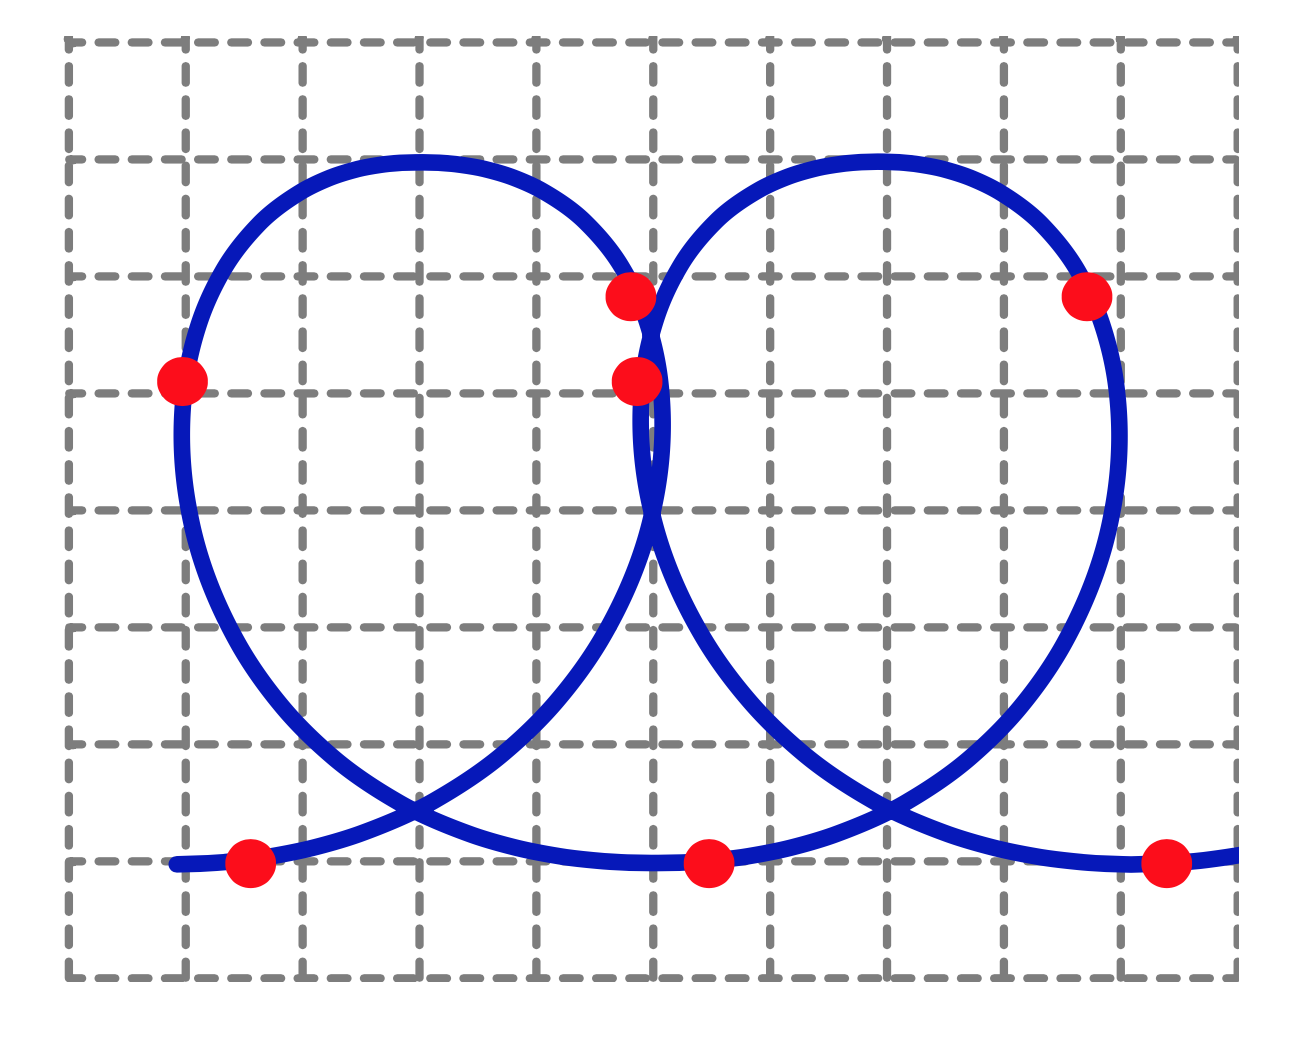
\includegraphics[scale = .2]{../tasks/kalda/rotdisk.png}
\end{minipage}
\begin{Answer}[ref = rotdisk]
	Es fällt auf, dass sich die blaue Bahn nach dem mittleren Punkt unten die Bewegung der Scheibe anscheind widerholt. Da bis dahin die Lampe genau drei Mal geblinkt hat, hat die Scheibe diese Strecke also in einer Zeit von 
	\begin{equation}\label{rotdisk:timeneed}
	T = 3t =0.3~\mathrm{sec}
	\end{equation}
	
	zurückgelegt, wobei $t = 0.1~\mathrm{sec}$ die Zeit ist, die zwischen dem Aufblinken der roten Lampe vergeht.\\
	Diese von der Scheibe zurückgelegte Strecke entspricht in etwa 4 Skaleneinheiten auf dem Bild. Gleichzeitig ist der Abstand zwischen dem untersten Punkt der blauen Bahn, und damit der untersten Position der Lampe, und dem obersten Teil der blauen Bahn, und damit der obersten Position der Lampe, 6 Skaleneinheiten lang. Aber der Abstand zwischen der obersten und der untersten Position der blauen Lampe entspricht genau $2a = 9~\mathrm{cm}$. Also ist eine Skaleneinheit genau $1.5~\mathrm{cm}$ lang. Somit ist die zurückgelegte Strecke $s = 6~\mathrm{cm}$. Für die Geschwindigkeit ergibt sich, mit\eqref{rotdisk:timeneed}
	\begin{equation}
	v = \frac{s}{T} =  \frac{6~\mathrm{cm}}{0.3~\mathrm{sec}} = 20~\mathrm{\frac{cm}{sec}}.
	\end{equation}
\end{Answer}
\begin{Exercise}[label = tempind, title = Temperaturunabhängiger Widerstand, difficulty = 2, origin = Alte IPhO-Aufgabe ]
Wir betrachten zwei Materialien $A$ und $B$, mit spezifischem Widerstand $\rho_A$ und $\rho_B$, die beide die gleiche Fläche haben. Die Temperaturkoeffizienten der beiden Widerstände sind $\alpha_A$ und $\alpha_B$, und geben an, um wieviel sich der Widerstand bei einer Temperaturänderung $\Delta T$ ändert. Es ist $\alpha_A < 0$ und $\alpha_B > 0$. \\
In welchem Längenverhältnis müssen die Längen der beiden Widerstände $\ell_A$ und $\ell_B$ stehen, damit der Gesamtwiderstand einer Reihenschaltung der beiden bei einer Temperaturänderung $\Delta T$ konstant bleibt?
\end{Exercise}
\begin{Answer}[ref=tempind]
Wenn die Temperaturänderung $\Delta T$ nicht zu groß ist, kann man den neuen Widerstand $R$ nach dieser Temperaturänderung aus dem alten Widerstand $R_0$ ausrechnen mit
\begin{equation}\label{tempunwds:rchange}
	R\left(\Delta T\right) = R_0 + \alpha \Delta T R_0 = R_0\left(1+\alpha \Delta T\right),
\end{equation}
wobei $\alpha$ der Temperaturkoeffizient ist.\\
Gleichzeit ist der Widerstand $R$ eines Körpers der Länge $\ell$, der Fläche $A$ und dem spezifischen Widerstand $\rho$ 
\begin{equation}\label{tempunwds:rdef}
	R = \frac{\rho \ell}{A}.
\end{equation}
Die zwei gegebenen Widerstände $R_A$ und $R_B$ sind in Reihe geschaltet, also ist der Gesamtwiderstand $R_g$ 
\begin{equation}\label{tempunwds:rg}
	R_g = R_A + R_B =\frac{1}{A}\left(\rho_A \ell_A + \rho_B \ell_B\right) 
\end{equation}
Wenn wir annehmen, dass die Temperaturänderung so klein ist, dass sich die Länge der Widerstände nicht ändert, können wir \eqref{tempunwds:rchange} genauso führ den spezifischen Widerstand schreiben
\begin{equation}\label{tempunwds:rhochange}
	\rho\left(\Delta T\right) = \rho_0 + \alpha \Delta T \rho_0 = \rho_0\left(1+\alpha \Delta T\right).
\end{equation}
Schreiben wir diesen Ausdruck nun für $R_A$ und $R_B$, so erhalten wir als Gesamtwiderstand in Abhängigkeit von der Temperatur aus \eqref{tempunwds:rg}
\begin{equation*}
	\tilde{R}_g\left(\Delta T\right) = \frac{1}{A}\left[\left(\rho_A + \rho_A \alpha_A \Delta T\right)\ell_A + \left(\rho_B + \rho_B \alpha_B \Delta T\right) \ell_B \right].
\end{equation*}
Ausklammern der Terme führt auf
\begin{equation}\label{tempunwds:rgtemp}
	\tilde{R}_g\left(\Delta T\right) =\underbrace{\frac{1}{A}\left[ \rho_A \ell_a + \rho_B \ell_B\right]}_{= R_g~  \mathrm{aus}~ \eqref{tempunwds:rg}} +\frac{\Delta T}{A} \left(\rho_A \alpha_A \ell_A + \rho_B \alpha_B \ell_B \right).
\end{equation}
Der erste Term ist genau der Gesamtwiderstand $R_g$ aus \eqref{tempunwds:rg} vor der Temperaturänderung. Der zweite Term ist ein Produkt aus $\Delta T$ und einem anderen Faktor. Damit der Gesamtwiderstand $\tilde{R}_g$ also unabhängig von der Temperaturänderung $\Delta T$ immer genau $R_g$ ist, muss der Faktor nach $\Delta T$ null sein, da dieser ganze Term dann keinen Einfluss hat. Also ist
\begin{equation}
\boxed{
	\rho_A \alpha_A\ell_A + \rho_B \alpha_B\ell_B = 0 \Rightarrow \frac{\ell_A}{\ell_B} = -\frac{\rho_B\alpha_B}{\rho_A\alpha_A}}.
\end{equation}
Das Minuszeichen muss da sein, da $\alpha_A$ auch negativ sein soll, und das Längenverhältnis nicht negativ sein sollte.
\end{Answer}


\end{document}